\documentclass[a4paper]{article}
\usepackage[spanish,activeacute]{babel}
\usepackage[ansinew]{inputenc}
% Anda fen'omeno mientras codifiquemos el archivo como ansi.
\usepackage{graphicx}
\usepackage[left=2cm,right=2cm]{geometry}
\usepackage{ulem} %Para tachar cosas
\usepackage{epigraph}
\usepackage{listings}
\usepackage{html}
\usepackage[colorlinks=true]{hyperref}
\parindent = 0 pt
\parskip = 11 pt

\newcommand{\haskell}{\textsl{Haskell}}
\newcommand{\hpage}{\textbf{\textsl{$\lambda$Page}}}
\newcommand{\cabal}{\textsl{Cabal}}

\begin{document}

    \thispagestyle{empty}
    \begin{center}
	    {\Large Tesis de Licenciatura}\\[1em]
	    {\huge \textbf{$\lambda$Page}}\\[0.5em]
	    {\large \textit{Un bloc de notas para desarrolladores Haskell}}\\[1em]
	    \par\vspace{\stretch{1}}
	    {\large Departamento de Computaci\'on}\\[0.5em]
	    {\large Facultad de Ciencias Exactas y Naturales}\\[0.5em]
	    {\large Universidad de Buenos Aires}
	    \par\vspace{\stretch{1}}
	    \begin{figure}[h]
	        \begin{center}
	        
\includegraphics[width=40mm]{logoUba}
	        \end{center}
	    \end{figure}
	    {\Large \textbf{Alumno}}\\[0.8em]
	    {\Large Fernando Benavides (LU 470/01)} \par
	    {\Large greenmellon@gmail.com} \par
	    \par\vspace{\stretch{1}}
	    {\Large \textbf{Directores}}\\[0.8em]
	    {\Large Dr. Diego Garbervetsky} \par
	    {\Large Lic. Daniel Gor'in} \par
	    \par\vspace{\stretch{2}}
         {\Large \textbf{Abstract}}\\[0.5em]
    \end{center}
    El presente documento describe una herramienta para desarrolladores \haskell\ que pretende facilitar la tarea de ``debuggear'', analizar y entender c'odigo, llamada \hpage.  Con ella el usuario puede manipular ``p'aginas'' de texto libre que contengan expresiones \haskell, intentar interpretar 'estas expresiones independientemente y analizar los resultados obtenidos.
    \vspace*{\stretch{3}}
    \newpage

\tableofcontents
\newpage

\section{Introducci'on}
\subsection{Motivaci'on}
\begin{epigraphs}
    \qitem{Motivation is what gets you started. Habit is what keeps you going}{Jim Rohn}
    \qitem{Essstamo mo-ti-va-dos, nene}{El ``Bambino'' Veira}
\end{epigraphs}
\paragraph{}Actualmente estamos presenciando un importante cambio en el desarrollo de sistemas, gracias al 'exito de proyectos como \htmladdnormallinkfoot{CouchDB}{http://couchdb.apache.org}, \htmladdnormallinkfoot{ejabberd}{http://www.ejabberd.im} y el chat de \htmladdnormallinkfoot{Facebook}{http://www.facebook.com}, todos ellos desarrollados utilizando lenguajes del paradigma funcional.
\paragraph{}Ejemplos de 'estos lenguajes de programaci'on, como \htmladdnormallinkfoot{Haskell}{http://www.haskell.org} o \htmladdnormallinkfoot{Erlang}{http://www.erlang.org}, demuestran ser maduros, confiables y presentan claras ventajas en comparaci'on con los lenguajes tradicionales del paradigma imperativo.  Sin embargo, los desarrolladores que deciden realizar el cambio de paradigma se encuentran con el problema de la escasez de ciertas herramientas que les permitan realizar su trabajo m'as eficientemente.  Por el contrario, 'estas herramientas abundan en el desarrollo de proyectos utilizando lenguajes orientados a objetos.  En particular, nuestro foco de atenci'on se centra sobre aquellas herramientas que permiten realizar \textsl{debugging} y \textsl{entendimiento} de c'odigo a trav'es de \textsl{``micro-testing''}\footnote{Enti'endase ``micro-testing'' como la tarea de realizar tests eventuales para entender o evaluar alg'un aspecto de un programa} .
\paragraph{}Los desarrolladores Haskell cuentan actualmente con dos herramientas de este tipo:
\begin{description}
	\item[\htmladdnormallinkfoot{GHCi}{http://www.haskell.org/ghc/docs/latest/html/users\_guide/ghci.html}]
		La consola que provee \htmladdnormallinkfoot{GHC}{http://www.haskell.org/ghc} permite a los desarrolladores evaluar expresiones, verificar su tipo o su clase.  Cuenta tambi'en con un \htmladdnormallinkfoot{mecanismo de debugging}{http://www.haskell.org/ghc/docs/6.10-latest/html/users\_guide/ghci-debugger.html} integrado que permite realizar la evaluaci'on de expresiones paso a paso.  Pese a ser la herramienta m'as utilizada por los desarrolladores, \textit{GHCi} tiene varias limitaciones.  En particular:
		\begin{itemize}
			\item No permite editar m'as de una expresi'on a la vez
			\item No permite intercalar expresiones con definiciones
			\item	Si bien permite utilizar definiciones, 'estas se pierden al recargar m'odulos
			\item No es sencillo utilizar en una sesi'on las definiciones y/o expresiones creadas en sesiones anteriores
		\end{itemize}
	\item[\htmladdnormallinkfoot{Hat}{http://www.haskell.org/hat}]
		Un herramienta para realizar seguimiento a nivel de c'odigo fuente.  A trav'es de la generaci'on de trazas de ejecuci'on, \textit{Hat} ayuda a localizar errores en los programas y es 'util para entender su funcionamiento.  Sin embargo, por estar basado en la generaci'on de trazas, requiere la compilaci'on y ejecuci'on de un programa para poder utilizarlo y esto no siempre es c'omodo para el desarrollador que puede querer simplemente analizar una expresi'on particular que incluso quiz'a no compile a'un.  Adem'as, su mantenimiento activo parece haber cesado hace m'as de un a'no y en su p'agina se observa una importante lista de \htmladdnormallinkfoot{problemas conocidos}{http://www.haskell.org/hat/bugs.html} y \htmladdnormallinkfoot{caracter'isticas deseadas}{http://www.haskell.org/hat/bugs.html}.  
\end{description}

%%------------------------------------------------------------------------------------------------------------------------------
\subsection{Trabajos Relacionados}
\begin{epigraphs}
	\qitem{If I have seen further it is only by standing on the shoulders of giants}{Isaac Newton}
	\qitem{I like work; it fascinates me. I can sit and look at it for hours}{Jerome Klapka}
\end{epigraphs}
\paragraph{}En el mundo de la programaci'on orientada a objetos podemos encontrar herramientas de este tipo, como \htmladdnormallinkfoot{Java Scrapbook Pages}{http://help.eclipse.org/help33/index.jsp?topic=/org.eclipse.jdt.doc.user/reference/ref-34.htm} para \htmladdnormallinkfoot{Java}{http://www.java.com} y \htmladdnormallinkfoot{Workspace}{http://wiki.squeak.org/squeak/1934} para \htmladdnormallinkfoot{SmallTalk}{http://www.smalltalk.org}.  Utilizando estos aplicativos, los desarrolladores pueden introducir peque'nas porciones de c'odigo, ejecutarlas y luego inspeccionar y analizar los resultados obtenidos.  Un concepto compartido por ambas herramientas es el de presentar ``p'aginas'' de texto en las que varias expresiones pueden intercalarse con partes de texto libre y permitir al desarrollador intentar evaluar s'olo una porci'on de todo lo escrito.  Estas p'aginas pueden ser guardardas y luego recuperadas de modo de poder analizar nuevamente las mismas expresiones.  Adem'as permiten crear objetos (lo que para los lenguajes funcionales equivaldr'ia a definir expresiones) locales a la p'agina en uso y utilizarlos en ella.
\paragraph{}Dentro del paradigma funcional, con un enfoque similar, aunque un poco m'as orientado a la presentaci'on y visualizaci'on de documentos, \htmladdnormallinkfoot{Keith Hanna}{http://www.cs.kent.ac.uk/people/staff/fkh/} de la Universidad de Kent, ha desarrollado \htmladdnormallinkfoot{Vital}{http://www.cs.kent.ac.uk/projects/vital/}.  \textsl{Vital} es una implementaci'on de un entorno de visualizaci'on de documentos para \haskell.  Pretende presentar \haskell\ de una manera apropiada para usuarios finales en areas de aplicaci'on como la ingenier'ia, las matem'aticas o las finanzas.  Dentro de esta herramienta, los m'odulos \haskell\ son presentados como documentos en los que pueden visualizarse los valores que en ellos se definen directamente en el lugar en el que aparecen, ya sea de modo textual o gr'afico (como ``vistas''). 
\paragraph{}Durante el desarrollo de \hpage\ hemos tenido que enfrentar varios desaf'ios relacionados principalmente con el desarrollo de interfaces visuales dentro del paradigma funcional.  Volcando el conocimiento adquirido durante ese proceso, hemos desarrollado \htmladdnormallinkfoot{wxhNotepad}{http://github.com/elbrujohalcon/wxhnotepad} que es, ante todo, una prueba de concepto sobre c'omo desarrollar editores de texto con \textsl{wxHaskell}.  Gracias a \htmladdnormallinkfoot{Jeremy O'Donoghue}{http://wewantarock.wordpress.com/about/}, \textsl{wxhNotepad} est'a siendo publicado como \htmladdnormallinkfoot{un tutorial}{http://wewantarock.wordpress.com/2010/01/31/building-a-text-editor-part-1/} en sucesivos art'iculos en su blog
%%------------------------------------------------------------------------------------------------------------------------------
\subsection{\hpage}
\begin{epigraphs}
    \qitem{Ancorch'e lo ingegno umano faccia invenzioni varie, rispondendo con vari strumenti a un medesimo fine, mai esso trover\`a invenzione pi\`u bella, n'e pi\`u facile n'e pi\`u brieve della natura, perch'e nelle sue invenzioni nulla manca e nulla \`e superfluo}{Leonardo da Vinci}
    \qitem{La programaci'on intensiva y el uso prolongado de Tetris s'olo lleva a ver estructuras de orden y secuencias en la verduler'ia y a querer apilar los autos para formar l'ineas s'olidas}{Dar'io Ruellan}
\end{epigraphs}
\paragraph{} \htmladdnormallinkfoot{\hpage}{http://haskell.hpage.com} se presenta como una herramienta  similar al Workspace de \textit{Smalltalk}, que permite a los desarrolladores trabajar con documentos de texto libre que incluyan expresiones y definiciones.  \hpage\ es capaz de identificar las expresiones y definiciones v'alidas y permite al desarrollador inspeccionarlas, evaluarlas, conocer su tipo y su clase.
\subparagraph{}En el esp'iritu de las herramientas provistas por la comunidad de desarrolladores \haskell, \hpage\ se integra con \htmladdnormallinkfoot{\cabal}{http://www.haskell.org/cabal} y \htmladdnormallinkfoot{Hayoo!}{http://holumbus.fh-wedel.de/hayoo} y se encuentra ya disponible en \htmladdnormallinkfoot{HackageDB}{http://hackage.haskell.org/package/hpage}.
\subparagraph{}\hpage\ presenta una interfaz simple e intuitiva, desarrollada utilizando \htmladdnormallinkfoot{wxHaskell}{http://haskell.org/haskellwiki/WxHaskell}, lo que lo convierte en un sistema multiplataforma.
\subparagraph{}Por ser una herramienta desarrollada con \haskell\ para \haskell, \hpage\ se diferencia de sus pares del mundo de objetos, al aprovechar conceptos claves como son el tipado fuerte (que permite detectar errores de tipo velozmente, evitando el costo de evaluar expresiones complejas) y la evaluaci'on perezosa (que permite evaluar expresiones infinitas e ir exhibiendo resultados progresivamente).
\subparagraph{}A diferencia de \textsl{GHCi} que es una herramienta ``de consola'', \hpage\ permite visualizar resultados de manera m'as din'amica, permitiendo que errores intermedios, detectados durante la evaluaci'on de una expresi'on no impidan continuar con la misma hasta llegar a un resultado m'as completo.
\subparagraph{}\hpage\ se encuentra desarrollado utilizando \htmladdnormallinkfoot{\textsl{eprocess}}{http://hackage.haskell.org/package/eprocess}, una librer'ia que facilita el manejo de ``threads'' en un estilo similar al de los procesos \textsl{Erlang}.  Gracias al uso de esta librer'ia, \hpage\ puede realizar tareas en paralelo y por lo tanto permitir al usuario continuar editando los documentos en los que est'a trabajando mientras espera que se eval'ue una expresi'on e incluso cancelar una evaluaci'on conservando la porci'on del resultado obtenida hasta ese momento.  Tambi'en gracias al uso de \textsl{eprocess}, \hpage\ permite detectar c'alculos infinitos (o m'as precisamente, c'alculos que demoran demasiado) e informar sobre este hecho al usuario para que ya no siga esperando indefinidamente el resultado de la evaluaci'on solicitada.
\newpage

\section{Tutorial - Descubriendo \hpage}
\subsection{Instalaci'on}
\begin{epigraphs}
	\qitem{As a rule, software systems do not work well until they have been used, and have failed repeatedly, in real applications.}{Dave Parnas}
	\qitem{The \#1 programmer excuse for legitimately slacking off: ``My code is compiling''}{David Knutz}
\end{epigraphs}
\paragraph{}Para instalar \hpage\ en \textsl{OSX} o \textsl{Windows}, se proveen instaladores en el sitio web de \hpage, sin embargo,como se ha dicho, \hpage\ se encuentra en \textsl{HackageDB} y por lo tanto el modo oficial de instalarlo es utilizando \cabal, con el siguiente comando:
\lstset{language=sh, frame=single, tabsize=2}
\begin{lstlisting}
$ cabal install hpage
\end{lstlisting}
\subparagraph{}Sin embargo, para ello, previamente se deben satisfacer las siguientes dependencias:
\begin{description}
	\item[\htmladdnormallinkfoot{wxWidgets 2.8.10+}{http://www.wxwidgets.org/downloads/}] El framework de desarrollo para interfaces de usuario que utiliza \textsl{wxHaskell}.  Debe ser instalado con los m'odulos unicode, cmdline, config, log, stl, richtext y clipboard, al menos y con el m'odulo odbc desactivado.
	\item[\htmladdnormallinkfoot{Haskell Platform}{http://hackage.haskell.org/platform/}] Una distribuci'on de \haskell\ que incluye todo lo necesario para compilar e instalar programas desarrollados en este lenguaje (de particular inter'es para \hpage: GHC y happy).
\end{description}
\subsubsection{Windows}
\paragraph{}Para el correcto funcionamiento de \hpage\ los usuarios de \textsl{Windows XP} deben instalar el \htmladdnormallinkfoot{C++ 2008 SP1}{http://www.microsoft.com/downloads/details.aspx?familyid=A5C84275-3B97-4AB7-A40D-3802B2AF5FC2}.
\subsubsection{Linux}
\paragraph{}En algunas distribuciones de Linux es conveniente, adem'as de la instalaci'on de \textsl{Haskell Platform} instalar las librer'ias de \textit{Monad Transformers} ejecutando, por ejemplo:
\begin{lstlisting}
$ sudo aptitude install libghc6-mtl-dev libghc6-mtl-doc
\end{lstlisting}
\newpage
\subsection{QuickStart}
\begin{epigraphs}
	\qitem{We learn by example and by direct experience because there are real limits to the adequacy of verbal instruction}{Malcom Gladwell}
	\qitem{How is education supposed to make me feel smarter? Besides, every time I learn something new, it pushes some old stuff out of my brain - remember when I took that home winemaking course, and I forgot how to drive?}{Homer Simpons}
\end{epigraphs}
TODO: Tutorial donde se noten las features de \hpage
\newpage

\section{Desarrollo - ?`C'omo se hizo \hpage?}
\subsection{Arquitectura General}
\begin{epigraphs}
	\qitem{If you think good architecture is expensive, try bad architecture}{Brian Foote and Joseph Yoder}
\end{epigraphs}
\paragraph{}Las principales decisiones de arquitectura que se tomaron durante el desarrollo de \hpage\ tuvieron como principales motivaciones los siguientes requerimientos:
\begin{description}
\item[Conexi'on con GHC] \hpage\ deb'ia conectarse con el motor de GHC a trav'es de su API de modo de poder detectar e interpretar expresiones.  Para ello se utiliz'o \htmladdnormallinkfoot{hint}{http://projects.haskell.org/hint}
\item[Paralelismo] \hpage\ deb'ia permitir al usuario editar sus documentos mientras esperaba el resultado de la evaluaci'on de alguna expresi'on.  Para ello se cre'o \textsl{eprocess} y se implement'o un modelo de procesos utiliz'andolo.
\item[Errores Controlados] \hpage\ no deb'ia fallar si la evaluaci'on de una expresi'on fallaba.  M'as a'un, tambi'en deb'ia detectar posibles evaluaciones infinitas e informar estas situaciones al usuario
\end{description}
\begin{figure}[hp]
	\begin{center}
        	\fbox{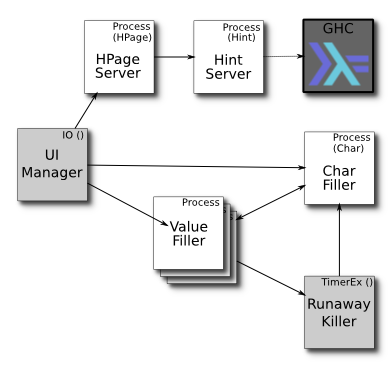
\includegraphics[]{architecture}}
		\caption{Arquitectura de \hpage}
		\label{arq1}
	\end{center}
\end{figure}
\subparagraph{}Teniendo en cuenta estos requerimientos, la arquitectura resultante puede ser descripta con el diagrama de la figura \ref{arq1}.  Esta figura presenta el estado del sistema en un instante dado.  Cada bloque representan un proceso o ``thread'' en ejecuci'on.  Cada uno de estos procesos se ejecuta dentro del entorno de una m'onada, la cual se encuentra identificada en la esquina superior derecha del bloque.  En el diagrama podemos identificar los siguientes componentes:
\begin{description}
	\item[UI Manager] Este es el thread que inicia el programa, genera y administra la interfaz del usuario utilizando las herramientas provistas por \textsl{wxHaskell}.  En este thread se mantiene el estado visual de la aplicaci'on: el estado de los controles, la 'ultima b'usqueda realizada, etc.
	\item[HPage Server] Este proceso, iniciado por el \textbf{UI Manager}, es el que comunica a la interfaz del usuario con la m'aquina virtual de GHC, a trav'es del \textbf{Hint Server}, captura sus errores y lo reinicia en caso de ser necesario.  En este proceso se mantiene el estado general de la aplicaci'on: sus p'aginas, expresiones, paquetes y m'odulos cargados, etc.
	\item[Hint Server] Este proceso, iniciado por el \textbf{HPage Server}, mantiene una conexi'on con la m'aquina virtual de GHC (a la cual se muestra en la figura conectado a trav'es de una l'inea de puntos)
	\item[Char Filler] Este proceso, iniciado por el \textbf{UI Manager} cumple una muy sencilla funci'on: utilizando los procedimientos de env'io y recepci'on de mensajes provistos por \textsl{eprocess}, espera recibir un caracter (o sea, una expresi'on de tipo Char), para luego evaluarlo y enviar como respuesta su valor en forma normal.
	\item[Value Filler] Estos procesos, iniciados por el \textbf{UI Manager} ante cada evaluaci'on solicitada por el usuario son los encargados de procesar el resultado obtenido del \textbf{HPage Server}. Cabe recordar aqu'i que \haskell\ trabaja con evaluaci'on ``lazy'', por lo cual el resultado obtenido no ha sido a'un completamente procesado.  Cada \textbf{Value Filler} se encarga de evaluar un resultado y mostrarlo por pantalla, para ello env'ia y recibe mensajes del \textbf{Char Filler} a fin de procesar cada caracter a mostrar.
	\item[Runaway Killer] Este thread, creado utilizando la clase \textsl{TimerEx} provista por \textsl{wxHaskell}, es iniciado por cada \textbf{Value Filler} al momento de enviar un nuevo caracter al \textbf{Char Filler}.  El objetivo del \textbf{Runaway Killer} es el de detectar prorcesamiento ``posiblemente'' infinito.  B'asicamente, pasado un segundo de procesamiento, reinicia el \textbf{Char Filler} e informa al \textbf{Value Filler} que lo inici'o que el caracter que se esperaba procesar ha demorado demasiado y podr'ia desencadenar una evaluaci'on infinita.
\end{description}
\paragraph{}Para un mayor detalle, la figura \ref{seq1} nos muestra un diagrama de secuencia correspondiente a un proceso de evaluaci'on.  Para poder brindar un ejemplo completo, hemos ``fabricado'' un tipo que responde al siguiente c'odigo:
\lstset{language=haskell, frame=single, tabsize=4}
\begin{lstlisting}
data WithIfiniteChar = WIC

instance Show WithIfiniteChar where
    show WIC = ['c', head . show $ length [1..]]
\end{lstlisting}
\subparagraph{}Como puede observarse, al intentar mostrar la expresi'on \texttt{WIC}, \hpage\ se encontrar'a con una cadena cuyo segundo caracter no puede computar pues requiere un c'alculo infinito, en la figura representamos este caracter con la letra $\Omega$.  All'i es donde entra en acci'on el \textbf{Runaway Killer} para informar esta situaci'on al usuario.
\begin{figure}[hp]
	\begin{center}
        	\fbox{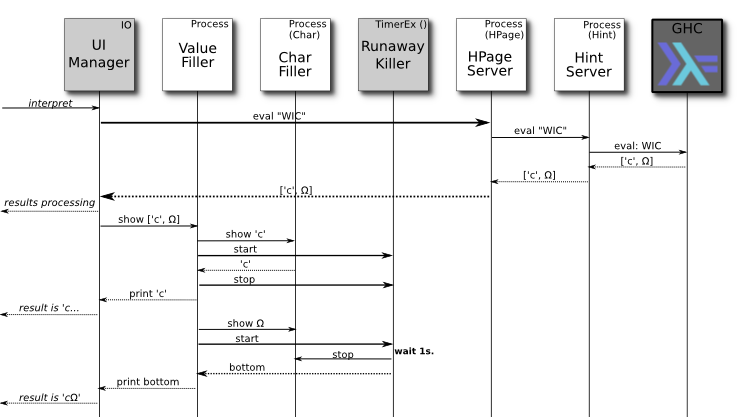
\includegraphics[width=\textwidth]{sequence}}
		\caption{Secuencia de Evaluaci'on de ``WIC''}
		\label{seq1}
	\end{center}
\end{figure}

\subsection{Dise'no}
\begin{epigraphs}
	\qitem{Design and programming are human activities; forget that and all is lost}{Bjarne Stroustrup}
\end{epigraphs}
\paragraph{}Presentaremos a continuaci'on las principales decisiones de dise'no que se han tomado durante la creaci'on de \hpage.  Todas ellas tienen como fundamento los requerimientos principales exhibidos en la secci'on anterior y tambi'en algunos requerimientos adicionales, como la integraci'on con \cabal\ y \textsl{Hayoo!}.
\subsubsection{Concurrencia}
\paragraph{}Como hemos visto en la secci'on anterior, al momento de dise'nar \hpage\ tuvimos que considerar la necesidad de paralelizar tareas, para permitir al usuario, por ejemplo, trabajar en un documento mientras el motor de \hpage\ eval'ua una expresi'on.  Tambi'en debemos considerar que estas tareas a realizar en paralelo no son totalmente independientes sino que requieren una sincronizaci'on.  Tomando la idea del modo en que est'a dise'nado el lenguaje de programaci'on \textsl{Erlang}, decidimos implementar el paralelismo utilizando lo que denominamos \textsl{procesos}.  Conceptualmente, los \textsl{procesos} son hilos de ejecuci'on que se realizan en paralelo y pueden recibir o enviar mensajes.   Esta caracter'istica de mensajer'ia entre procesos es la que permite la sincron'ia cuando es necesaria.  Por otra parte, a diferencia de \textsl{Erlang}, al utilizar \haskell, los mensajes enviados de un proceso a otro pueden ser mucho m'as complejos.  Gracias al uso de m'onadas, un proceso puede enviar a otro directamente las acciones que desea que 'este ejecute, tal como deben ser ejecutadas.  Esta es una caracter'istica esencial para reducir la complejidad de la implementaci'on de todos nuestros procesos, en particular de aquellos que act'uan como servidores (\textbf{HPage Server} y \textbf{Hint Server}), como veremos luego en la secci'on \textsl{Implementaci'on}.
\subsubsection{Bottoms}
\paragraph{}El lenguaje \haskell\ tiene una caracter'istica 'unica: \textsl{la evaluaci'on perezosa} o \textsl{lazy evaluation}.  Gracias a esta caracter'istica, las expresiones \haskell\ no son completamente evaluadas (reducidas a forma normal) hasta el momento en que realmente se necesita conocer su valor.  Dado que \hpage\ presenta al usuario un interprete de expresiones, es necesario que est'e preparado para no s'olo soportar sino tambi'en aprovechar esta caracter'istica.  En particular, dentro de \hpage\ las expresiones son reducidas a forma normal al momento de intentar mostrar el resultado de su evaluaci'on al usuario.  En ese momento, lo 'unico que se sabe es que la expresi'on a mostrar es de clase \textsl{Show}.  \hpage\ intenta entonces ejecutar la funci'on \texttt{show} sobre la expresi'on a mostrar y pueden suceder varias cosas:
\begin{itemize}
	\item Por supuesto, puede suceder que al evaluar la expresi'on se obtenga una cadena de caracteres, en cuyo caso \hpage\ simplemente presentar'a el resultado al usuario
	\item Puede suceder que, intentando evaluar la expresi'on se obtenga una cadena de caracteres de longitud infinita.  La pol'itica de \hpage\ en este caso es permitir al usuario decidir cu'ando desea abortar la evaluaci'on y mostrar la porci'on del resultado obtenida hasta ese momento
	\item Puede suceder tambi'en que, intentando evaluar un caracter, se genere un c'alculo ``infinito'' o una excepci'on.  En este caso, \hpage\ aborta el proceso que se encuentra intentando evaluar el caracter en cuesti'on e informa este hecho al usuario, para luego continuar evaluando los siguientes caracteres
	\item Otra posibilidad es que, luego de presentar un caracter, al intentar obtener el resto de la cadena, \hpage\ encuentre un c'alculo ``infinito'' o una excepci'on.  En estos casos, se informa la situaci'on al usuario y se aborta la evaluaci'on de la expresi'on.
\end{itemize}
\subsubsection{Integraci'on}
\paragraph{}Una de las herramientas m'as comunmente usada por los desarrolladores haskell es \cabal.  \cabal\ (Common Architecture for Building Applications and Libraries) es una API distribuida con GHC que permite a un desarrollador agrupar f'acilmente un conjunto de m'odulos para producir un paquete. Es el sistema de compilaci'on est'andar para las aplicaciones y librer'ias de \haskell.  En un \textsl{paquete Cabal}, el desarrollador define los m'odulos que componen su aplicaci'on o librer'ia, los lugares (carpetas) donde encontrar el c'odigo fuente y los recursos que 'estos necesitan para funcionar, junto con las extensiones que se requieren para poder compilarlos.
\subparagraph{}\hpage\ por su parte, permite al desarrollador cargar o importar m'odulos para poder utilizarlos al momento de evaluar expresiones.  Tambi'en permite definir los lugares donde el compilador puede encontrar archivos fuentes y las extensiones que 'este debe utilizar al momento de compilar los archivos encontrados.
\subparagraph{}Observando estas similitudes, una integraci'on con \cabal\ es algo que surge de manera natural y \hpage\ lo provee.  \hpage\ permite al desarrollador cargar un paquete \cabal\ previamente configurado y de ese modo utilizar los m'odulos, extensiones y ubicaciones en el definidos.
\paragraph{}Otra herramienta, quiz'a no tan popular como \cabal, pero tambi'en muy 'util es \textsl{Hayoo!}.  \textsl{Hayoo!} es un motor de b'usqueda especializado en la documentaci'on de la API de \haskell.  El objetivo de \textsl{Hayoo!} es proporcionar una interfaz de b'usqueda interactiva y f'acil de usar para la documentaci'on de varios paquetes y librer'ias \haskell.  Conociendo esta herramienta, decidimos integrarla con \hpage\ de modo que el desarrollador pueda realizar consultas en su base de datos para obtener informaci'on sobre alguna funci'on, tipo, m'odulo, clase o expresi'on que desee analizar.

\subsection{Implementaci'on}
\begin{epigraphs}
	\qitem{Nothing resolves design issues like an implementation}{J. D. Horton}
	\qitem{A child of five would understand this. Send someone to fetch a child of five}{Groucho Marx}
\end{epigraphs}

\subsubsection{eprocess}
\paragraph{}Para la implementaci'on de \textsl{eprocess}, nuestra librer'ia de procesos, utilizamos dos herramientas de paralelismo y concurrencia que se encuentran muy bien descriptas en el libro \htmladdnormallinkfoot{Real World Haskell}{http://book.realworldhaskell.org/read/concurrent-and-multicore-programming.html}.  Utilizamos \textsl{Threads} para paralelizar procesos y \textsl{Channels} y \textsl{MVars} para permitirles comunicarse.  Definimos entonces un tipo mon'adico para representar a las acciones a realizarse en procesos paralelos de tipo \texttt{m}, tales que retornan expresiones de tipo \texttt{a} y pueden recibir elementos de tipo \texttt{r}:
\begin{lstlisting}
newtype ReceiverT r m a = RT { internalReader :: ReaderT (Handle r) m a }
    deriving (Monad, MonadIO, MonadTrans, MonadCatchIO)
\end{lstlisting}
\subparagraph{}Individualizamos luego este tipo gen'erico, definiendo el tipo \texttt{Process}:
\begin{lstlisting}
type Process r = ReceiverT r IO
\end{lstlisting}

\subparagraph{}Finalmente definimos las funciones que permiten la ejecuci'on y mensajer'ia entre procesos:
\begin{lstlisting}
type Process r = ReceiverT r IO
\end{lstlisting}

TODO: Escribir m�s...

\subsubsection{UI}
\paragraph{}La interfaz gr'afica de \hpage\ est'a desarrollada utilizando \textsl{wxHaskell}, un framework elegido por ser multi-plataforma y, gracias a estar constru'ido sobre \textsl{wxWidgets}, presentar un ``look\&feel'' nativo en distintos entornos.  \textsl{wxHaskell} es un framework sencillo para utilizar y entender y, pese a que a'un se encuentra en per'iodo de evoluci'on, es suficientemente estable.  Sin embargo, tal como puede verse en \textsl{wxhNotepad} hemos tenido que superar varios escollos hasta lograr una UI estable e intuitiva.  A los lectores interesados en estos detalles t'ecnicos les recomendamos la lectura de los art'iculos escritos por Jeremy O'Donoghue en su tutorial \ \htmladdnormallinkfoot{Building a text editor}{http://wewantarock.wordpress.com/2010/01/31/building-a-text-editor-part-1/}.
\subsubsection{TODO: OTROS}
\paragraph{}TODO: Ver el c'odigo... detectar cosas interesantes y armarles secciones

\section{Resultados}
\subsection{Objetivos Alcanzados}
\begin{epigraphs}
	\qitem{Results! Why, man? I have gotten a lot of results. I know several thousand things that wont work}{Thomas A. Edison}
	\qitem{Kids, you tried your best and you failed miserably. The lesson is: ``never try''}{Homer Simpsons}
\end{epigraphs}
TODO: ?`Qu'e se puede hacer ahora que existe \hpage?
\subsection{Trabajo a Realizar}
\begin{epigraphs}
	\qitem{Inside every large program, there is a small program trying to get out}{C.A.R. Hoare}
	\qitem{I'm a man with a one-track mind, so much to do in one life-time}{Queen}
\end{epigraphs}
So much to do, so little done, such things to be
TODO: Future Work

\section{Agradecimientos}
\paragraph{}TODO: Acknowledgments.  Recordar a Jeremy, al flaco del Undo/Redo, a los de Hayoo!
\end{document}